\chapter{研究の準備}\label{cha:Preparation}
本章では、本研究で必要となる前提知識を説明する。
% \section{モータ作成}\label{motor}
% \subsection{仕様書}\label{siyo}
% \subsection{シミュレータの役割}\label{simu}
\section{Modelica言語}\label{modelica}
Modelica言語とは、微分代数方程式を用いた、複合領域のマルチドメインモデリングのために開発されたオブジェクト指向言語である\cite{modelicaモデルベース本}。
その言語仕様は、非営利団体のModelica Associationが策定している。
Modelica Associationでは、Modelica言語による様々な物理領域のモデルライブラリを開発しており、
数学、機械、電気、熱、流体、制御系、状態遷移機械などを含んだフリーのModelica標準ライブラリ(Modelica Standard Library : MSL)をリリースしている
\cite{modelicaモデルベース本}。
\section{OpenModelica}\label{OM}
OpenModelicaとは、Open Source Modelica Consortium (OSMC)が開発しているModelicaコードのモデリング、シミュレーション、デバッグのための機能などを
持つオープンソースプラットフォームである\cite{fritzson2006openmodelica}。
OpenModelicaでは、シミュレーション結果をグラフとして画面上に描画できる。また、シミュレーション結果は、以下の3つのファイル形式から保存することができる。
\begin{itemize}
    \item matファイル
    \item pltファイル
    \item csvファイル
\end{itemize}

今回試作するモータ特性表自動生成ツールでは、csvファイルにのみ対応する。

OpenModelicaから出力されるcsvファイルの一部を、図\ref{fig:simyu_csv}に示す。

図\ref{fig:simyu_csv}に示すcsvファイルの1列目には、時間を表すデータが必ず入る。
そして1列目の「time」を除いて1行目には、オブジェクト名を含んだ変数名が必ず入る。

OpenModelicaから出力されるcsvファイルのファイル名は、「(シミュレーションしたモデルの名前)\_res.csv」で生成される。
もし、シミュレーションしたモデルの名前が、「hoge」だった場合、csvファイルのファイル名は「hoge\_res.csv」となる。\\
\begin{figure}[t]
	\centering
	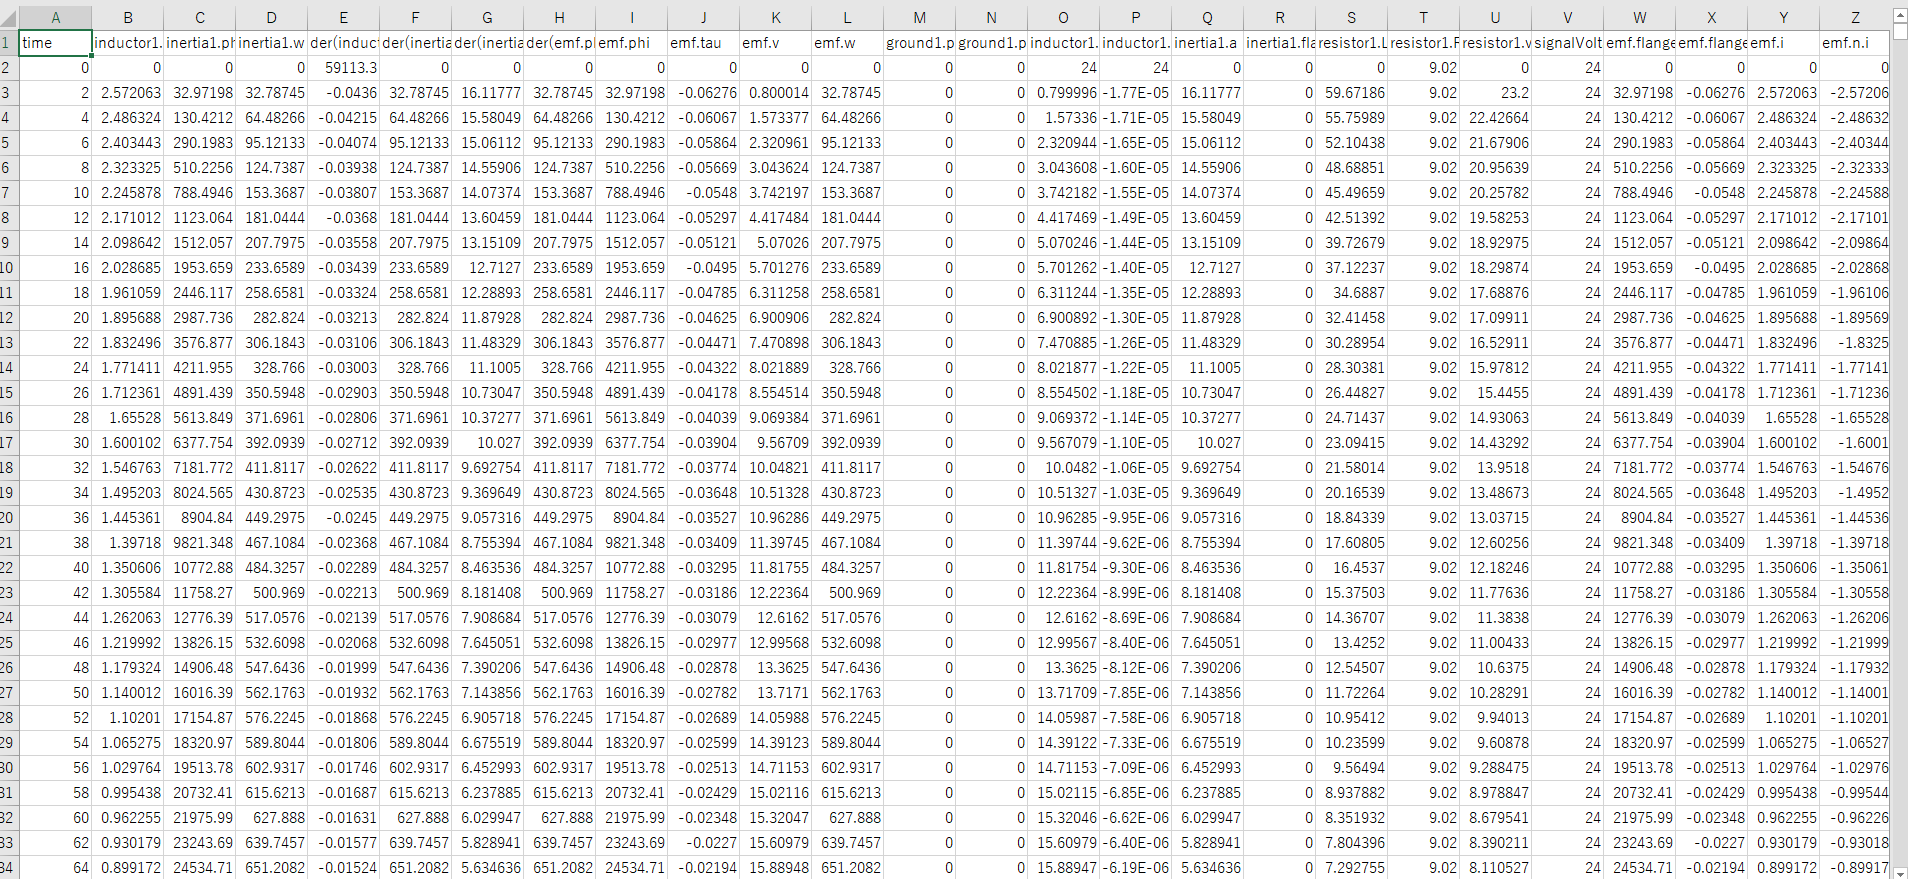
\includegraphics[width=16.5cm,height=10cm]{./Image/simyu_csv.png}
	\caption{シミュレーション結果のcsvファイルの一部}
	\label{fig:simyu_csv}
\end{figure}
% 試作するモータ特性表自動生成ツールでは、OpenModelica 1.9.1 Beta1を使用する。
\section{ブラシ付きDCモータ}\label{}
% ブラシ付きDCモータだけかけばいいのか?モータ全体の話も必要か?
ブラシ付きDCモータとは、磁場の中にあるコイルに電流を流す事で発生するローレンツ力を回転方向に利用することで回すモータである\cite{モータ原理}。
シンプルな構造で、制御しやすく、汎用性が高く、模型用モータや自動車補機用モータなど世界で一番多く使われているモータである\cite{モータ使う}。
% 3章へ
%   今回試作するモータ特性表自動生成ツールでは、ブラシ付きモータのシミュレーション結果にのみ対応する。
\section{対応するモデル}\label{taioumodel}
試作するモータ特性表自動生成ツールでは、以下2つのModelicaモデルのシミュレーション結果に対応する。
% \begin{itemize}
% 	\item ブラシ付きDCモータのModelicaモデル
% 	\item ブラシ付きDCモータのModelicaモデルをサブシステムとするモデル
% \end{itemize}
% 以降、上記のモデルについて具体的に説明する。
\subsection{ブラシ付きDCモータのModelicaモデル}\label{sub:tanntai}
ブラシ付きDCモータのModelicaモデルとは、ブラシ付きDCモータの等価回路\cite{等価回路}をModelica言語で表したモデルのことである。

ブラシ付きDCモータの等価回路をModelica言語で表すためには、電源部品、抵抗部品、インダクタ部品、起電力部品、慣性部品、接地部品が必要である。
% 上記6つの部品が必要な理由は、ブラシ付きDCモータの等価回路\cite{等価回路}をModelica言語で表す際に、使用する部品\cite{modelicaシステム本}だからである。\\

また、電源部品、抵抗部品、インダクタ部品、起電力部品、慣性部品には、それぞれ以下のパラメータを設定しなければならない。
\begin{itemize}
	\item 電源部品 ・・・ 電圧値 V
	\item 抵抗部品 ・・・ 抵抗値 $\Omega$
	\item インダクタ部品 ・・・ インダクタンス値 H
	\item 起電力部品 ・・・ トルク定数 $\mathrm{N\cdot m/A}$
	\item 慣性部品 ・・・ 慣性モーメント $\mathrm{kg\cdot m^2}$
\end{itemize}

各部品で使用するMSLを表\ref{tab:MSL}に、ブラシ付きDCモータの等価回路を図\ref{fig:touka}に、ブラシ付きDCモータのModelicaモデルの例を図\ref{fig:tantai_model}に、
図\ref{fig:tantai_model}のModelicaコードを図\ref{fig:tantai_modelica}に、それぞれ示す。

\begin{table}[t]
	\centering
	\caption{MSL対応表}
	\begin{tabular}{|c|c|} \hline
	  部品名 & 使用するMSL \\ \hline \hline
	  電源部品 & Modelica.Electrical.Analog.Sources \\ \hline
	  抵抗部品 & Modelica.Electrical.Analog.Basic \\ \hline
	  インダクタ部品 & Modelica.Electrical.Analog.Basic \\ \hline
	  起電力部品 & Modelica.Electrical.Analog.Basic \\ \hline
	  慣性部品 & Modelica.Mechanics.Rotational.Components \\ \hline
	  接地部品 & Modelica.Electrical.Analog.Basic \\ \hline
	\end{tabular}
	\label{tab:MSL}
  \end{table}
 
\begin{figure}[t]
	\centering
	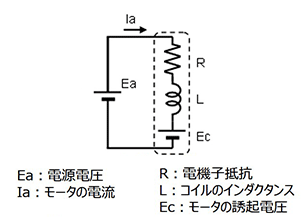
\includegraphics[width=7cm]{./Image/touka.png}
	\caption{ブラシ付きDCモータの等価回路}
	\label{fig:touka}
  \end{figure}

\begin{figure}[t]
  \centering
  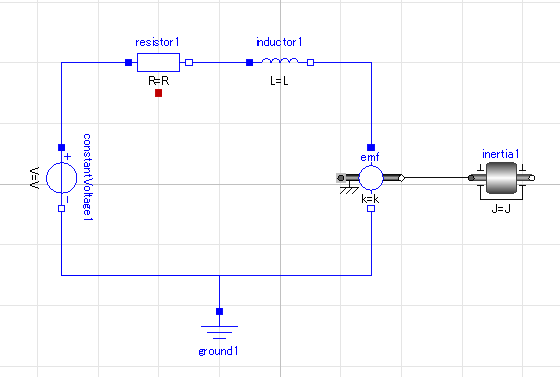
\includegraphics[width=10cm]{./Image/tantai_model.png}
  \caption{ブラシ付きDCモータのModelicaモデルの例}
  \label{fig:tantai_model}
\end{figure}


% \begin{figure*}[t]
% 	\lstinputlisting[label={code:motor}, caption={図\ref{fig:tantai_model}のModelicaコード}]{./chapters/motor.mo}
% \end{figure*}

\begin{figure}[t]
	\centering
	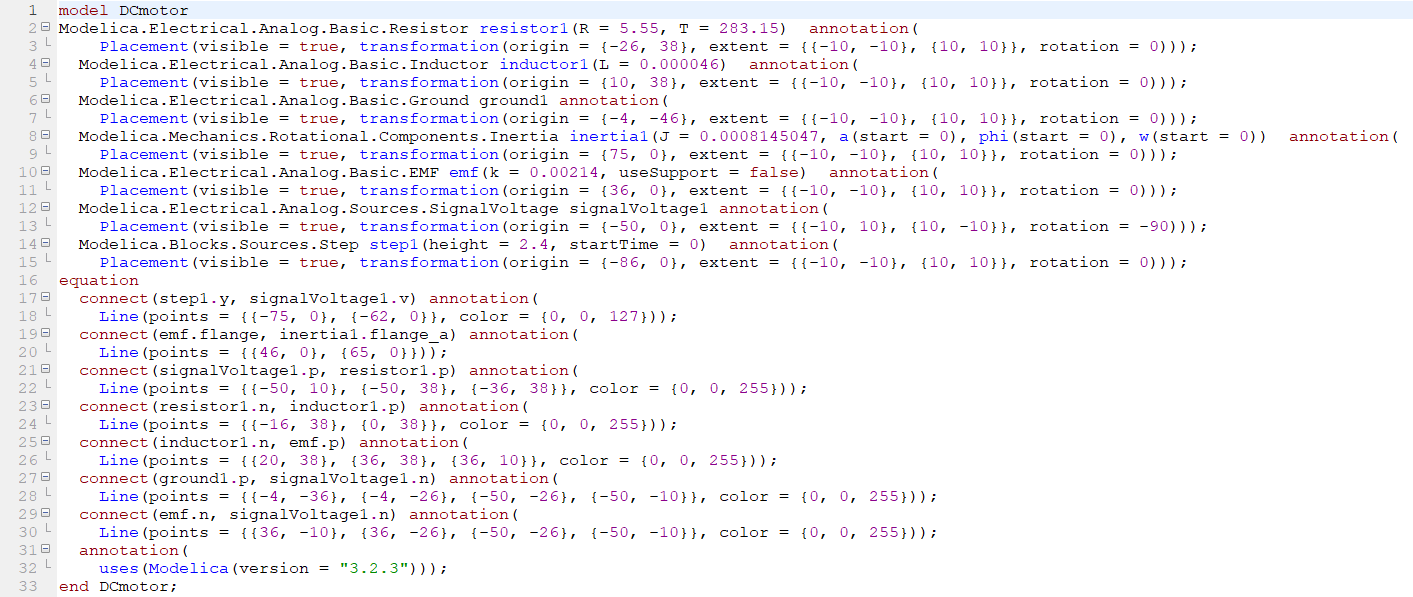
\includegraphics[width=16.5cm,height=8cm]{./Image/tantai_modelica.png}
	\caption{図\ref{fig:tantai_model}のModelicaコード}
	\label{fig:tantai_modelica}
  \end{figure}

%   \vspace{-1zh}

\subsection{ブラシ付きDCモータのModelicaモデルをサブシステムとするモデル} \label{sub:submodel}
ブラシ付きDCモータのModelicaモデルをサブシステムとするモデルとは、
\ref{sub:tanntai}節で説明したブラシ付きDCモータのModelicaモデルを1つのサブシステムとして扱い、他の部品と合わせたモデルのことである。

例として、ブラシ付きDCモータのサブシステムを用いたDCモータサーボのモデルを図\ref{fig:submodel}に、図\ref{fig:submodel}のModelicaコードを図\ref{fig:sub_modelica}に、それぞれ示す。

\begin{figure}[t]
	\centering
	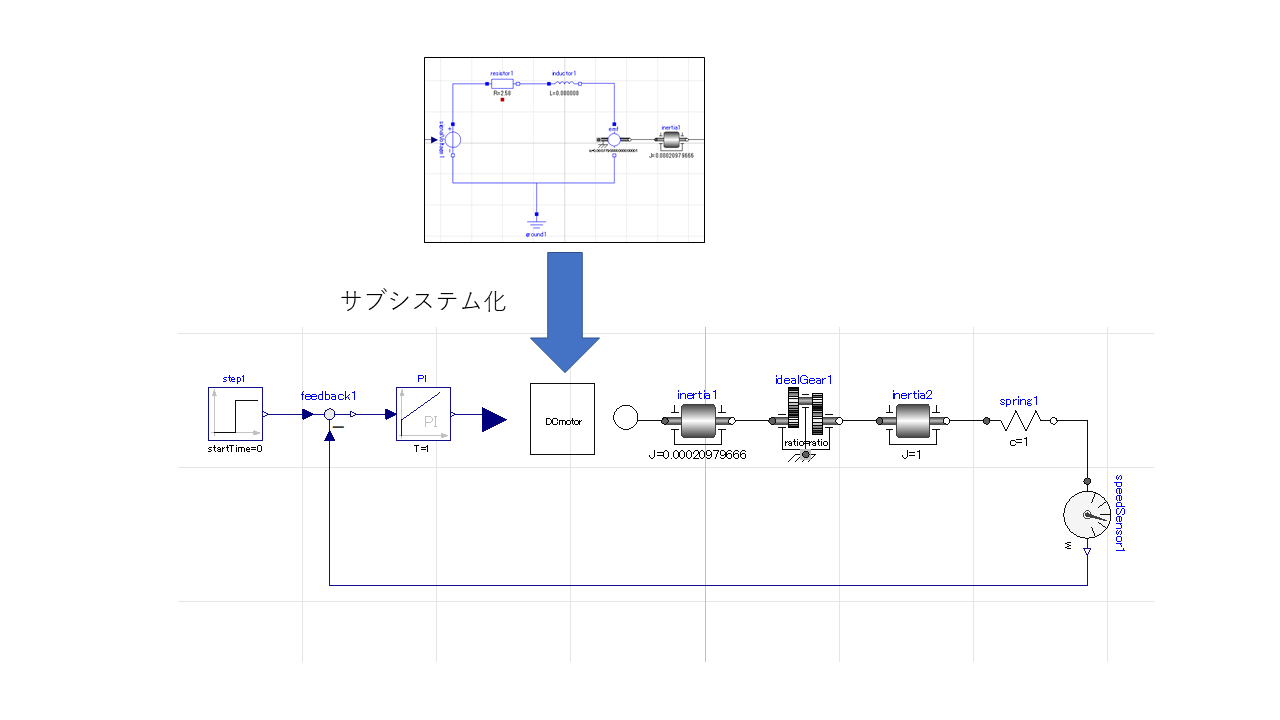
\includegraphics[width=16.5cm,height=10cm]{./Image/submodel_pack.png}
	\caption{DCモータサーボのモデル}
	\label{fig:submodel}
  \end{figure}

  \begin{figure}[t]
	\centering
	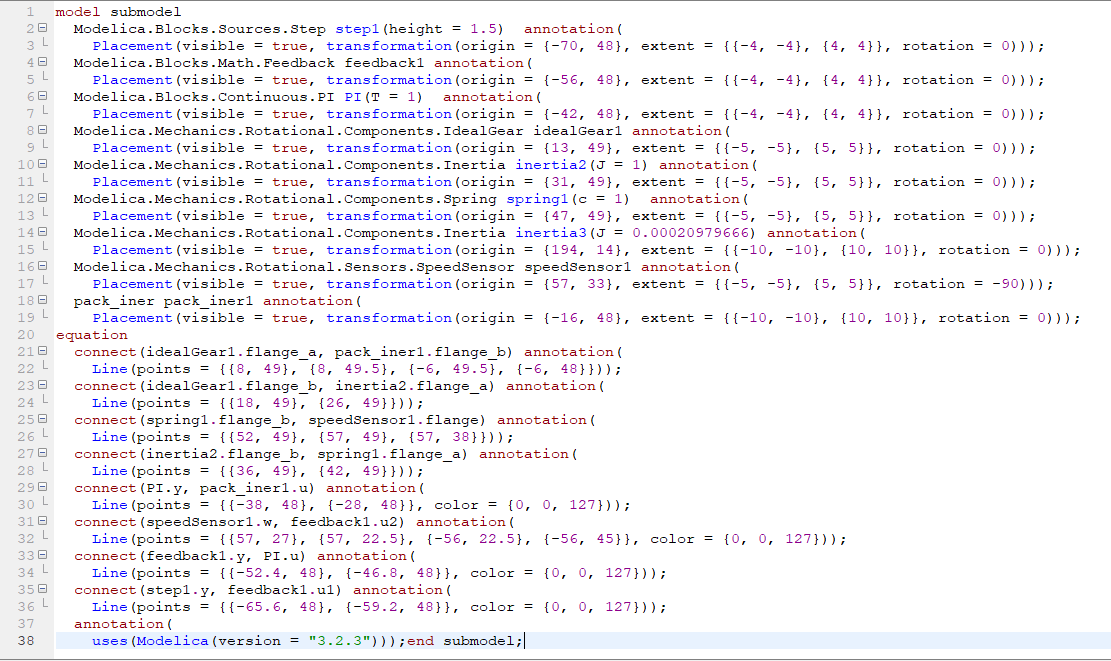
\includegraphics[width=16.5cm,height=10cm]{./Image/sub_modelica.png}
	\caption{図\ref{fig:submodel}のModelicaコード}
	\label{fig:sub_modelica}
  \end{figure}
% 3章へ
%   \subsection{モデル作成時の制約}\label{sub:seiyaku}
%   \ref{sub:tanntai}章、\ref{sub:submodel}章で説明したモデルを作成する際は、以下の制約を満たしていなければならない。
% \subsubsection{電圧値は一定}
% 今回試作するモータ特性表自動生成ツールでは、電圧値が一定の場合に得られる特性\cite{電圧一定}も示すため、入力である電圧値は一定でなければならない。
% \subsubsection{0秒からモータを動かす}
% 今回試作するモータ特性表自動生成ツールの仕様上、モータに対して0秒から入力を与え、モータを動かすようにしなければならない。
\section{モータ特性表}\label{mortoku}
モータ特性表とは、モータを選定する際に、参考にする資料である\cite{仕様の見方}。一般的に決まった形式はなく、企業によって書いている要素は異なるため、
10社のモータ特性表\cite{特性表1,特性表2,特性表3,特性表4,特性表5,特性表6,特性表7,特性表8,特性表9,特性表10}に書かれている要素を集計した。その中でも出現回数が多く、
ブラシ付きDCモータのシミュレーション結果から作成できる要素を、今回自動生成するモータ特性表の要素とした。

以下にモータ特性表の構成と要素を示す。
% \begin{itemize}
% 	\item モータ特性表
% 	\begin{itemize}
% 		\item 特性表
% 		\begin{itemize}
% 			\item 電圧 V
% 			\item 始動電流 mA
% 			\item 停動トルク $mN \cdot m$
% 			\item 最大効率 \%
% 			\item 定格トルク $mN \cdot m$
% 			\item 定格回転数 rpm
% 			\item 定格電流 mA
% 			\item 定格出力 W
% 			\item 最大回転数 rpm 
% 		\end{itemize}
% 		\item 特性グラフ
% 		\begin{itemize}
% 			\item トルク $mN \cdot m$ * 電流 mA
% 			\item トルク $mN \cdot m$ * 回転数 rpm
% 			\item トルク $mN \cdot m$ * 効率 \%
% 			\item トルク $mN \cdot m$ * 出力 W
% 		\end{itemize}
% 	\end{itemize}
% \end{itemize}
\subsection{特性表}\label{sub:tokuseihyou}
特性表を構成する9個の要素が表す内容について述べる。
% \begin{itemize}
% 	\item 電圧 V
% 	\item 始動電流 mA
% 	\item 停動トルク mNm
% 	\item 最大効率 \%
% 	\item 定格トルク mNm 
% 	\item 定格回転数 rpm
% 	\item 定格電流 mA
% 	\item 定格出力 W
% 	\item 最大回転数 rpm 
% \end{itemize}
% 以降、各要素が表す内容について述べる。
\subsubsection{電圧}\label{sub:sub:dennatu}
% \subsection{電圧}\label{sub:dennatu}
電圧とは、シミュレーション時に、回路に印加された電圧値を表す。

単位は、V(ボルト)である。
\subsubsection{始動電流}\label{sub:sub:sidouden}
% \subsection{始動電流}\label{sub:sidouden}
始動電流とは、モータの起動時に流れる電流値を表す。

単位は、mA(ミリアンペア)である。
% https://www.tsugawa.co.jp/glossary/ 
\subsubsection{停動トルク}\label{sub:sub:teidoutoruku}
% \subsection{停動トルク}\label{sub:teidoutoruku}
停動トルクとは、モータが出しうる最大トルクで、このトルク以上の負荷がかかれば、モータが停止する値を表す。

単位は、mNm(ミリニュートンメートル)である。
% https://www.orientalmotor.co.jp/tech/glossary/ta11/
\subsubsection{最大効率}\label{sub:sub:saidaikouritu}
% \subsection{最大効率}\label{sub:saidaikouritu}
効率とは、入力電力に対する機械出力の比を百分率[\%]で表したものであり、最大効率は、その中で最大値を表す。

単位は、\%(パーセント)である。
% https://www.jp-igarashi.com/product/product_motors/curve.html
\subsubsection{定格トルク}\label{sub:sub:teikakutoruku}
% \subsection{定格トルク}\label{sub:teikakutoruku}
定格トルクとは、最大効率時のトルク値を表す。

単位は、mNM(ミリニュートンメートル)である。
% http://www.sagamimicro.co.jp/product/aboutusage.html
\subsubsection{定格回転数}\label{sub:sub:teikakukaiten}
% \subsection{定格回転数}\label{sub:teikakukaiten}
定格回転数とは、最大効率時の回転数値を表す。

単位は、rpm(アールピーエム)である。

% https://mathwords.net/kaitensu
\subsubsection{定格電流}\label{sub:sub:teikakuden}
% \subsection{定格電流}\label{sub:teikakuden}
定格電流とは、最大効率時の電流値を表す。

単位は、mA(ミリアンペア)である。
% http://fa-faq.mitsubishielectric.co.jp/faq/show/18504?category_id=1937&site_domain=default
\subsubsection{定格出力}\label{sub:sub:teikakusyutu}
% \subsection{定格出力}\label{sub:teikakusyutu}
定格出力とは、最大効率時の出力値を表す。

単位は、W(ワット)である。
% \ref{sub:sub:teikakukaiten}章で求めた定格回転数と\ref{sub:sub:teidoutoruku}章で求めた定格トルクを
% http://www.nidec-servo.com/jp/digital/pdf/A_technique.pdf
\subsubsection{最大回転数}\label{sub:sub:saidaikai}
% \subsection{最大回転数}\label{sub:saidaikai}
最大回転数とは、回転数値の中で最大値を表す。

単位は、rpm(アールピーエム)である。
\subsection{特性グラフ}\label{sub:tokuseigurahu}
今回試作したツールでは、以下の4つの特性グラフを作成する。
% \begin{itemize}
% 	\item トルク mNM * 電流 mA
% 	\item トルク mNm * 回転数 rpm
% 	\item トルク mNm * 効率 \%
% 	\item トルク mNm * 出力 W
% \end{itemize}
% 以降、各グラフについて述べる。
\subsubsection{「トルク * 電流」グラフ}\label{sub:sub:torden}
「トルク * 電流」グラフとは、横軸が「トルク mNm」、縦軸が「電流 mA」のグラフである。\\
このグラフでは、トルクに対する電流の変化量を表している。
\subsubsection{「トルク * 回転数」グラフ}\label{sub:sub:torkaiten}
「トルク * 電流」グラフとは、横軸が「トルク mNm」、縦軸が「回転数 rpm」のグラフである。\\
このグラフでは、トルクに対する回転数の変化量を表している。
\subsubsection{「トルク * 効率」グラフ}\label{sub:sub:torkouritu}
「トルク * 電流」グラフとは、横軸が「トルク mNm」、縦軸が「効率 \%」のグラフである。\\
このグラフでは、トルクに対する効率の変化量を表している。
\subsubsection{「トルク * 出力」グラフ}\label{sub:sub:torsyutu}
「トルク * 電流」グラフとは、横軸が「トルク mNm」、縦軸が「出力 W」のグラフである。\\
このグラフでは、トルクに対する出力の変化量を表している。
  \section{Python}\label{python}
Pythonは、1991年にオランダ人のグイド・ヴァンロッサムというプログラマによって開発され、オープンソースで運営されている動的プログラミング言語である\cite{pythonoya}。
一括りにPythonといってもその用途は様々で、組み込み開発や、Webアプリケーション、デスクトップアプリケーション、さらには人工知能開発、ビッグデータ解析などと多岐に渡る\cite{pythonsamu}。
Pythonのプログラミング言語としての主な特徴は、少ないコードで簡潔にプログラムを書けること、専門的なライブラリが豊富にあることなどが挙げられる。

% pythonのバージョンは3.8.0
今回試作するモータ特性表自動生成ツールの開発言語に、Pythonを用いる。
また、使用するライブラリを以下に示す。
\begin{itemize}
	\item csv
	\item math
	\item matplotlib
	\item numpy
	\item decimal
	\item reportlab
	\item PIL
	\item pdf2image
	\item sys
	\item time
	\item os
\end{itemize}
% avaは、1990年代前半にSun MicrosystemsでJames Arthur Gosling、Wiliam Nelson Joyなどの人々が開発したプログラミング言語およびプラットフォームである。
% Javaはクラスベースのオブジェクト指向プログラミング言語である。
% Javaのプログラムは複数のクラスから構成され、クラス定義からそのクラスのインスタンスであるオブジェクトを何個でも作ることができる%\cite{プログラミング言語Java}。

% 1つのjavaファイルには複数のクラスを記述できる。
% 各クラスにはメンバが存在し、メンバの主な種類はフィールドとメソッドである。
% フィールドは、クラス自身あるいはそのクラスのオブジェクトのどちらかに属しているデータ変数である。
% メソッドは、クラスの状態を操作するためにフィールドに対して実行可能な処理を行う振舞いである。

% 今回実装は、で開発する。